\section{Component Division}
\label{design:division}

As described in \autoref{related:ondemand} on page \pageref{related:ondemand}, the proposed architecture initially only envisioned one bootware component.
This architecture was expanded with the introduction of the provisioning manager, as described in \autoref{related:dynamic} on page \pageref{related:dynamic}.
At this stage, the provisioning manager included all the functionality necessary to provision and deprovision provisioning engines in the cloud, in addition to the functionality already mentioned in \autoref{related:dynamic}.
This was a somewhat convoluted design where multiple responsibilities where mixed into one component.
It was later decided that the provisioning manager should be split into two parts.
The actual provisioning manager handles the communication with the service repository and the various provisioning engines, as described before in \autoref{related:dynamic}.
A separate bootware component handles the provisioning and deprovisioning of the provisioning engines.
At the moment, that leaves us with two bootware components, one local and one remote, where the local bootware component kick-starts the remote bootware, which then handles the actual provisioning of provisioning engines.
The first question that has to be answered is whether or not this division is reasonable, or if another alternative makes more sense.
We will now discuss the viability of four such alternatives.

\subsection{Single Local Component}

\begin{figure}[!htbp]
	\centering
	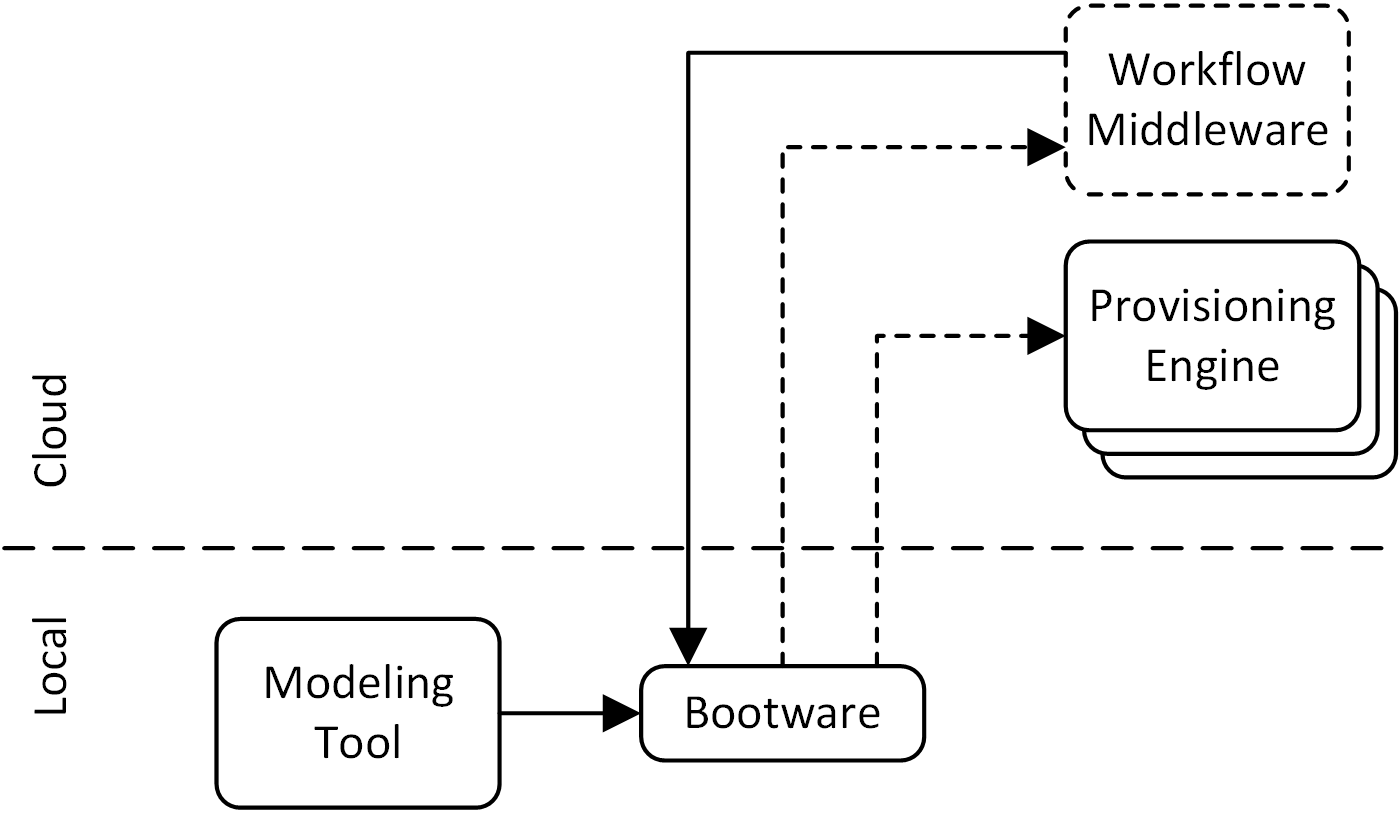
\includegraphics[resolution=600]{design/assets/simple_local}
	\caption{Simplified overview of the single local component architecture}
	\label{image:single_local}
\end{figure}

First we consider the simplest case: A single local component.
In this scenario, all provisioning processes are initiated from a component installed locally on the users machine, alongside or as part of the workflow modeler.

The advantages of this architecture lie in its simplicity.
Only one component has to be created and managed.
We wouldn't have to deal with any cloud environments and each user would have his own personal instance, so multi-tenancy wouldn't be an issue.
There is no possible overlap in functionality, as it would be the case in a 2-tier architecture (see \autoref{design:division:2tier}) and communication between multiple bootware components doesn't have to be considered.

The disadvantages are caused by the component being local.
Since all the functionality is concentrated in one component, it can become quite large and complicated, which is one thing that should be avoided according to the requirements.
A much bigger problem however is the remote communication happening in this scenario.
All calls to the bootware component from the ESB of the workflow middleware would leave the remote environment.
Also, all calls from the bootware component to the provisioning engines would enter the remote environment.
This type of split communication can be costly and slow, as shown by Li et al.
They compared public cloud providers and measured that intra-datacenter communication can be two to three times faster and also cheaper (often free) compared to inter-datacenter communication~\autocite{cloudcmp}.

\subsection{Single Remote Component}

\begin{figure}[!htbp]
	\centering
	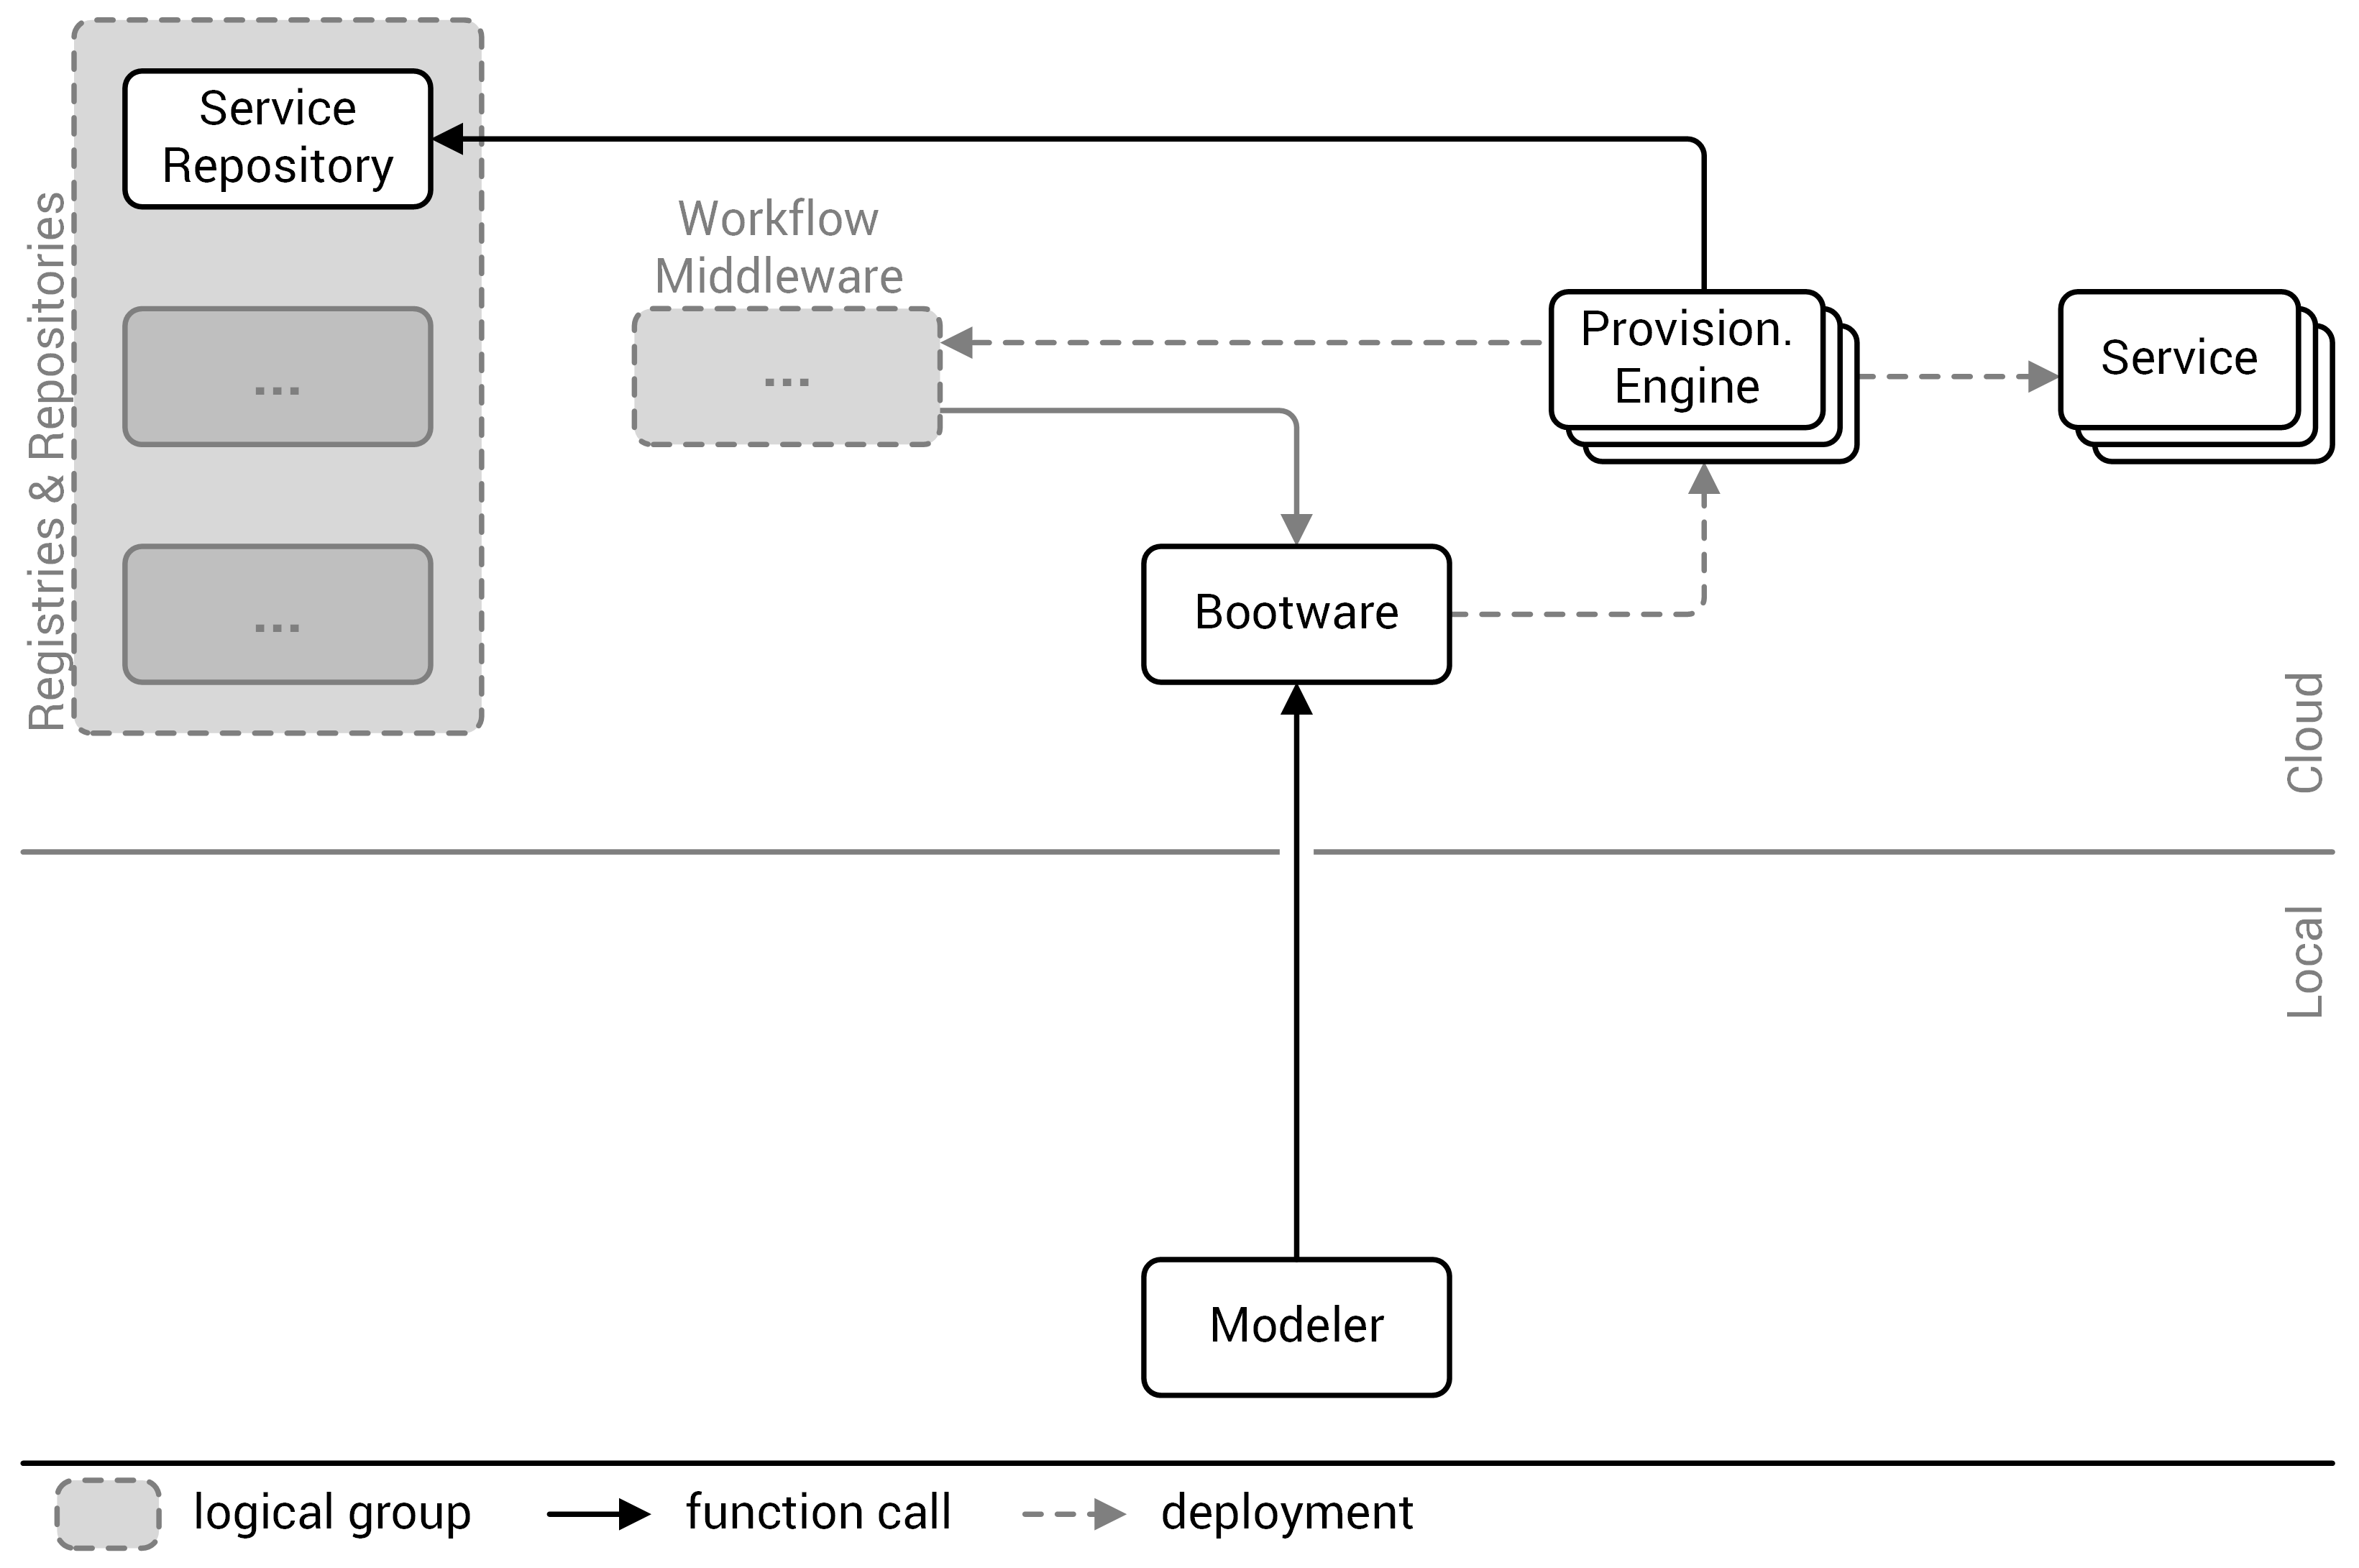
\includegraphics[resolution=600]{design/assets/simple_remote}
	\caption{Simplified overview of the single remote component architecture}
	\label{image:single_remote}
\end{figure}

The next obvious choice is to put the single bootware component into a remote environment, where the disadvantages of local to remote communication would disappear.
However, this creates new problems.

Since there aren't any additional components in this scenario that could manage the life-cycle of the remote bootware, the user would have to manage it by hand, which leads to two possibilities.
Either the user provisions the bootware once in some cloud environment and then keep this one instance running, or she provision it once she needs it and deprovisions it when she is done.

In the first case the user would only have to provision the bootware once, but this creates a new problem: The user doesn't know where exactly to put the bootware component.
Since one requirement is that multiple cloud environments should be supported, it is possible that the bootware component is not located anywhere near the cloud environment where it should provision further components.
The communication problem of the single local bootware component can still occur in these cases.

Another problem is that the bootware would be running all the time, even if the user doesn't need it, which would increase costs.
This problem could be reduces if this bootware instance is shared with others to assure a more balanced load.
But then the user would have to manage some sort of load balancing and the bootware component would have to support multi-tenancy or be stateless to be able to cope with potential high usage spikes.
This would further complicate the design and implementation of the bootware component and possibly increase the running costs.

In the second case the user would provision the bootware whenever she needs it. Now the user would be able to pick a cloud environment that is close to the other components that she plans to provision later.
This eliminates the two major problems of the first case but increases the effort that the user has to put into a task that she shouldn't have to do in the first place.
Life-cycle management of the bootware should be automated completely and hidden away from the user.
Therefor, this scenario is not appropriate for our case.

\subsection{2-Tier Architecture}
\label{design:division:2tier}

\begin{figure}[!htbp]
	\centering
	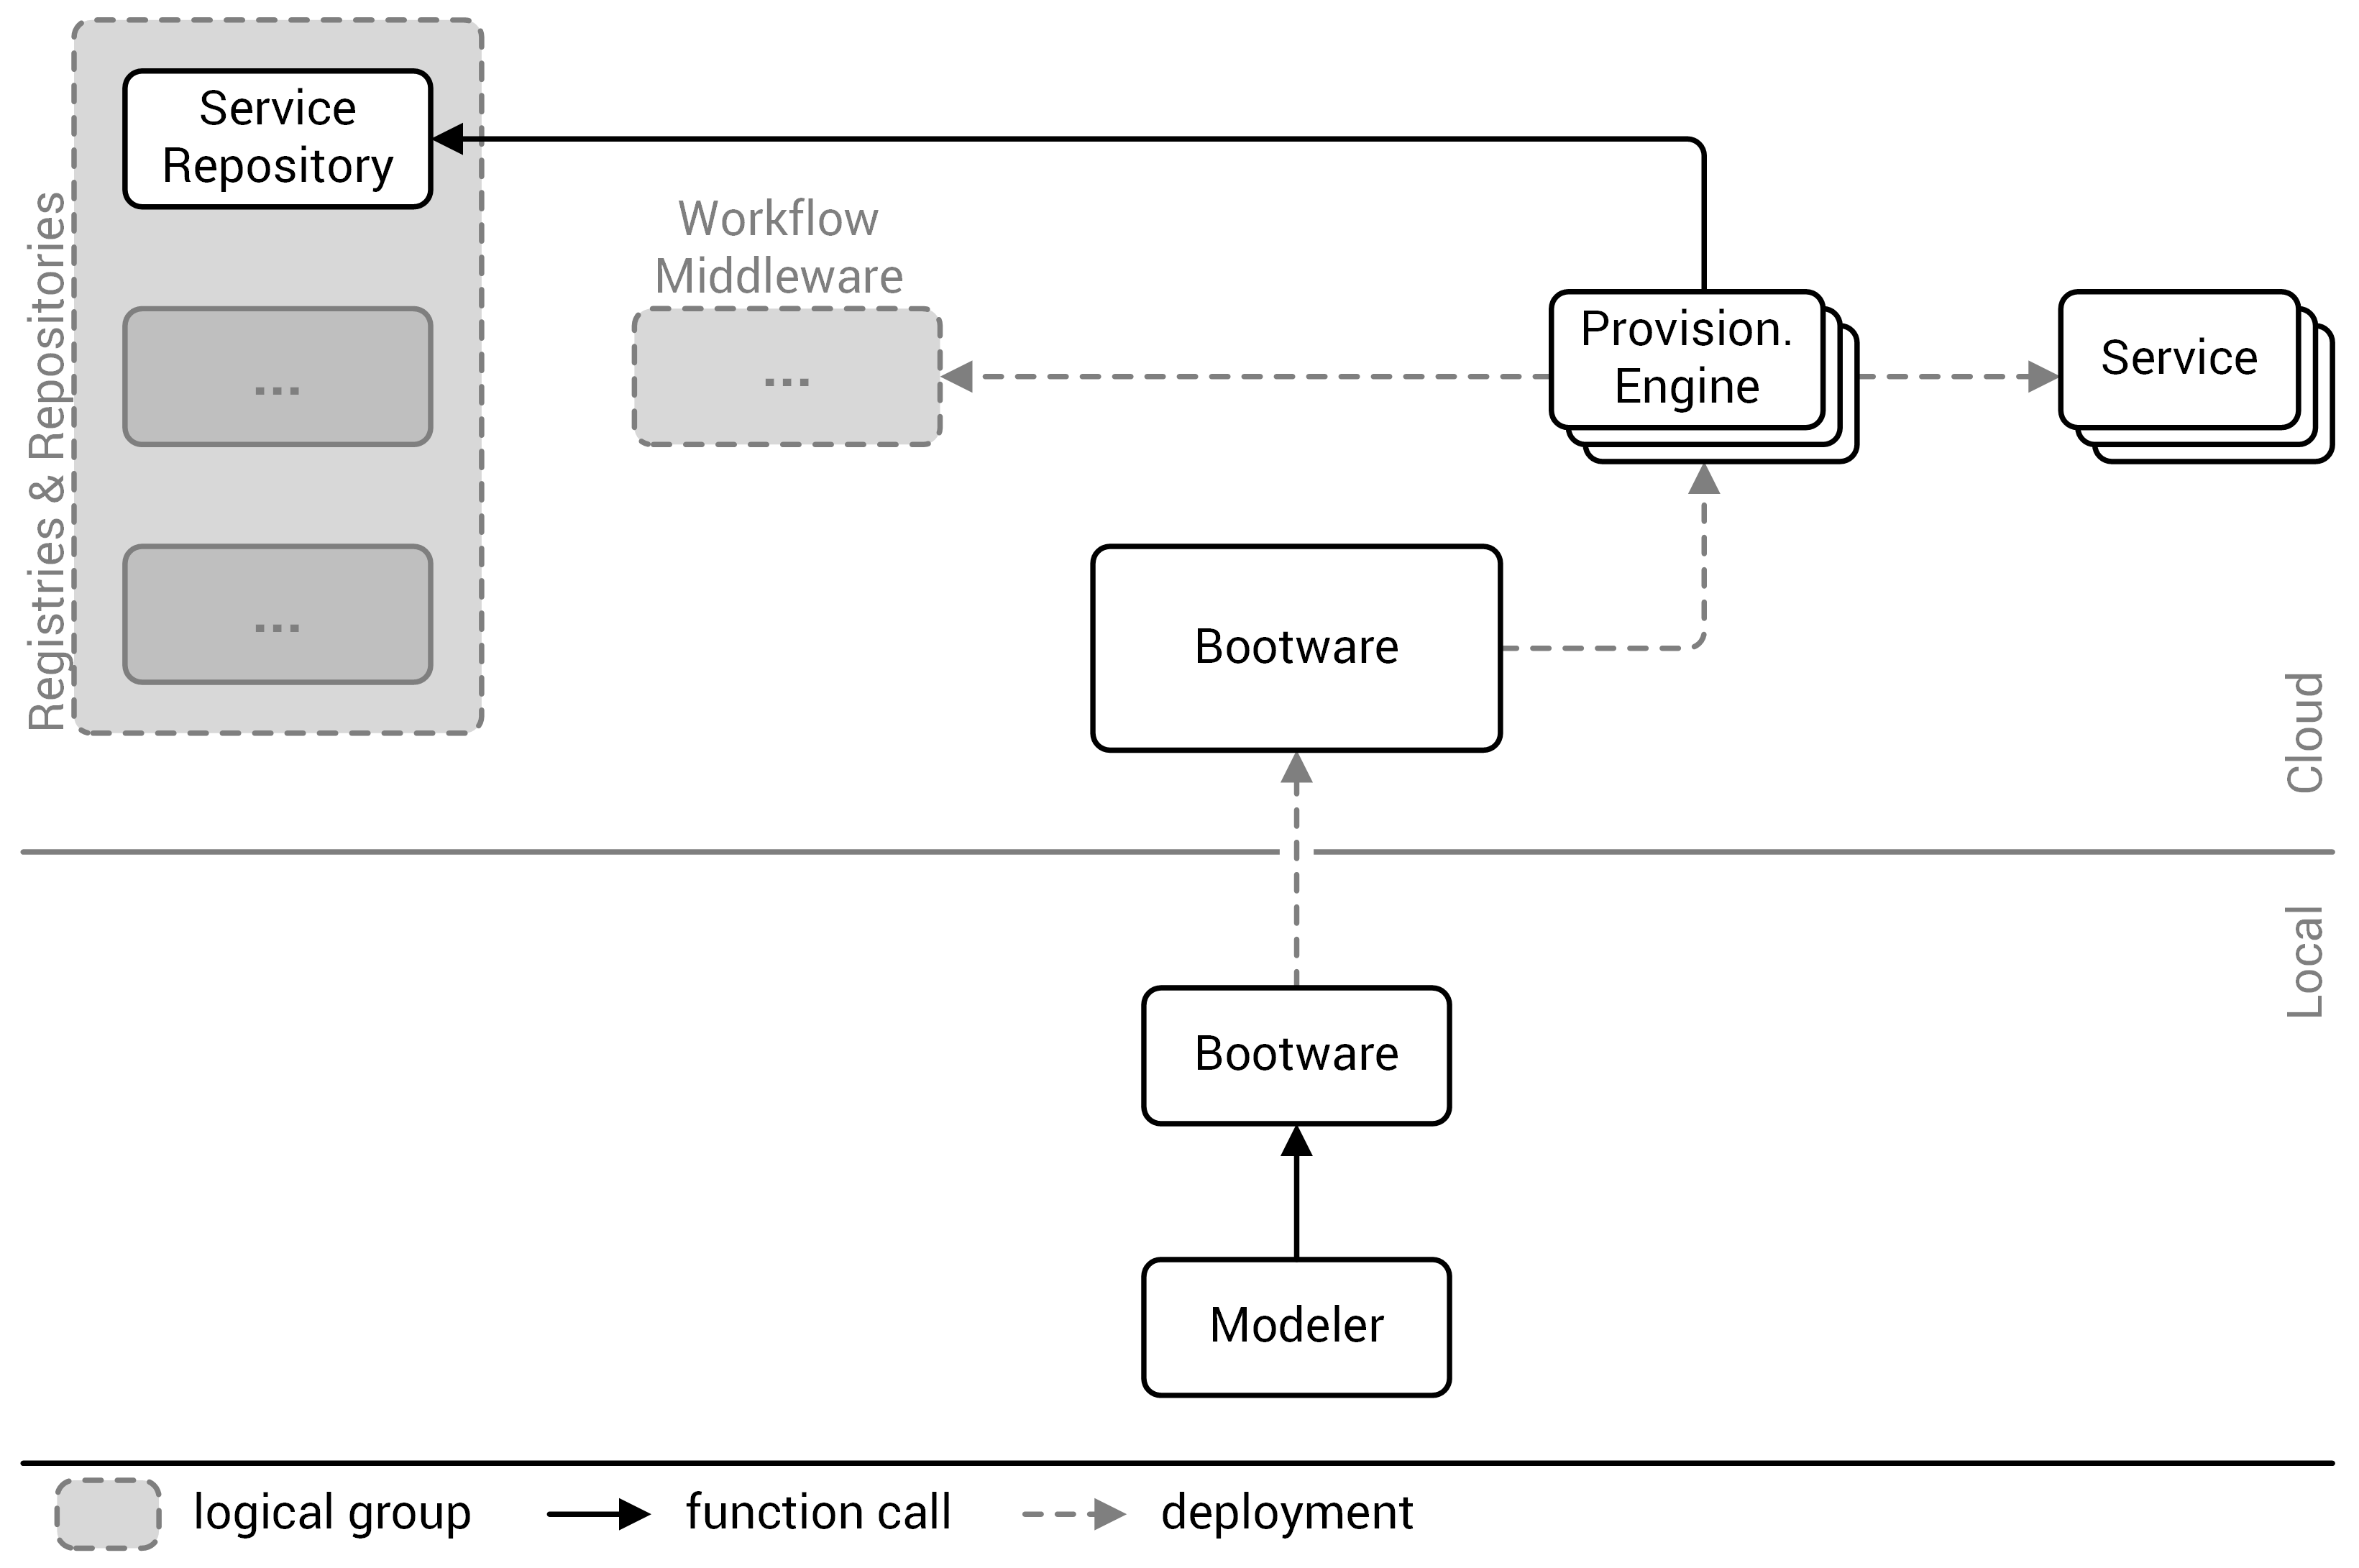
\includegraphics[resolution=600]{design/assets/simple_2_tier}
	\caption{Simplified overview of the 2-tier architecture}
	\label{image:2_tier}
\end{figure}

Next, we take a look at a 2-tier architecture, where the bootware is divided into two components.
On the local side we have a small and simple component which has mainly one function: To provision the larger second part of the bootware in a remote environment near to the environment, where other components will be provisioned later.

This eliminates the problems of a single local or remote bootware component.
The user no longer has to be involved in the management of the remote bootware since the local bootware handles all that.
Since we provision the remote bootware on demand we now also can position the remote bootware close to other remote components to minimize local/remote communication and the problems resulting of it.
We can now keep the local part as simple as possible and make the remote part as complicated as it has to be and since we provision the remote bootware only for one user we don't have to worry about multi-tenancy.

But we also introduce new problems.
For one, we now have duplicate functionality between the two components.
Both components have to know how to provision a component into multiple cloud environments.
The local component has to be able to put its remote counterpart into any cloud environment.
The remote component has to be able to provision other components into the same environment in which it runs (ideally, to minimize costs).
Since itself can be located in any cloud environment, it has to be able to do this in any cloud environment.
Independent from this, it has to be able to provision to any environment that the user/service package chooses.
But this problem can be solved by using a plugin architecture, which allows both components to use the same plugins.
We discuss plugins in detail in \autoref{design:extensibility}.

A second problem which we can't avoid but can solve is the communication which is now necessary between the different parts of the bootware.
More on this in \autoref{design:communication}

\subsection{Cloning}

\begin{figure}[!htbp]
	\centering
	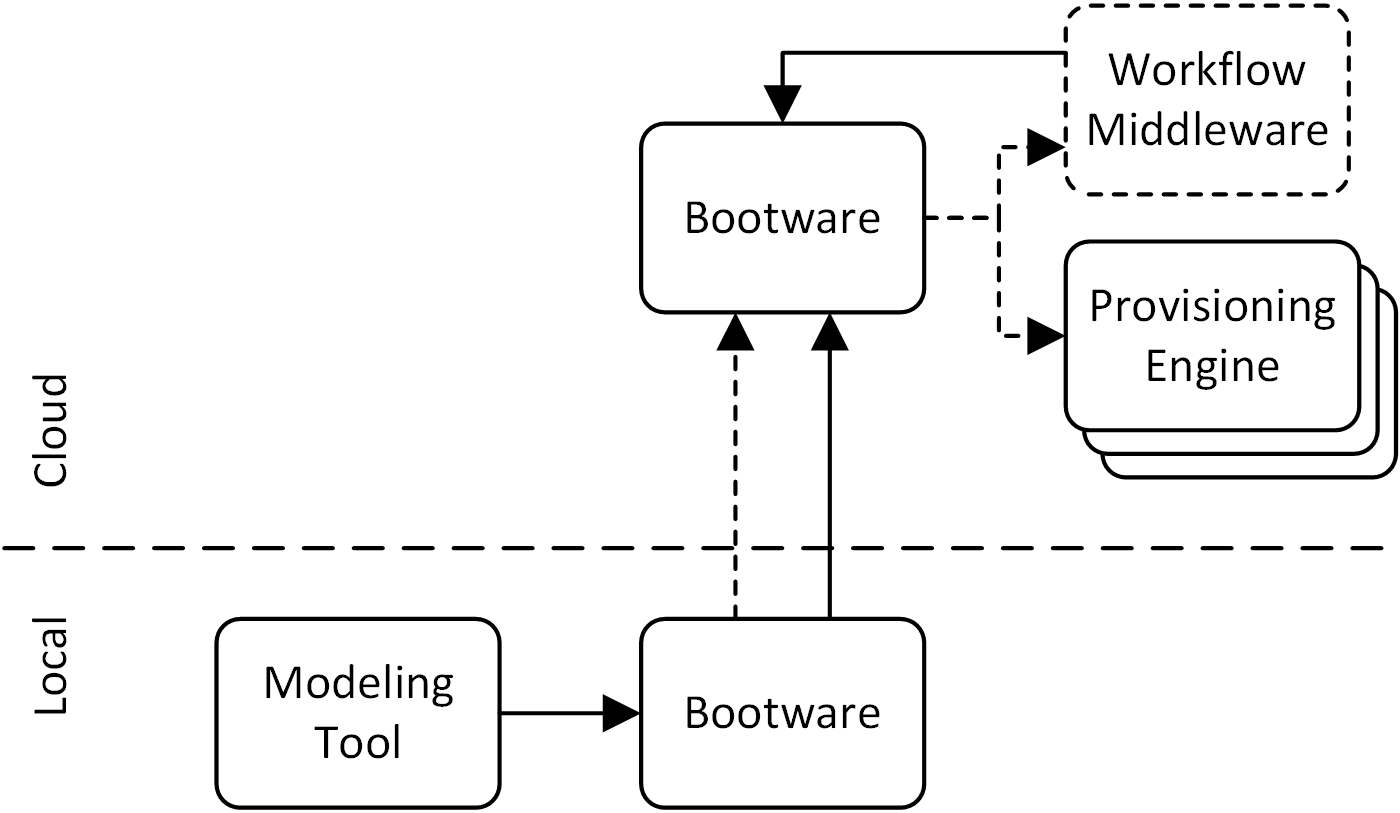
\includegraphics[resolution=600]{design/assets/simple_clone}
	\caption{Simplified overview of the cloned component architecture}
	\label{image:clone}
\end{figure}

This architecture can be seen as an alternative form of the 2-tier architecture described in \autoref{design:division:2tier}.
In this case there are also two bootwares working together and the remote bootware does most of the work.
However, the local and the remote bootware are identical.
Instead of provisioning a bigger bootware in a remote environment, the local bootware clones itself.
Compared to the 2-tier architecture described before, this has the advantage that only one component has to be designed and implemented and that function duplication is not an issue.
The disadvantage would be that the local bootware would be exactly as complex as the remote bootware and would contain functionality that it wouldn't require for local operation (e.g. a web service interface).
However, since we want to keep the whole bootware, including the remote part, fairly lightweight, it's highly unlikely that the complexity of the remote bootware will reach such heights that it could not be run on an average local machine.
In this case, the advantage of only having to design and implement one component seems to outweigh the disadvantage of a slightly more complex local component (compared to the 2-tier variant).
Of course, this architecture makes only sense if the functionality of the two separate components in the 2-tier architecture turns out to be mostly identical.
Therefore we can't decide yet if this architecture should be used.

\subsection{Decision}

Of the four alternative presented here, alternative three - the 2-tier architecture - makes the most sense.
Therefore it is selected as the alternative of choice and used for further discussion.
We do however retain the option to transform it into alternative four if we discover that both components share much of same functionality, but this can only be judged at a later stage, when we know exactly how the internal functionality of the bootware will work.
